%   % !TEX root = ../../VIII,3_Rahmen-TeX_8-1.tex
%
%
%   Band VIII, 3 N.~??S01.04
%   Signatur/Tex-Datei: LH_35_09_23_007-008
%   RK-Nr. 41208 /4
%   \ref{dcc_03}
%   Überschrift: De corporum concursus scheda tertia
%   Modul: Mechanik / Stoß ()
%   Datierung: Januar 1678
%   WZ: LEd-WZ 803003 = RK-WZ 142 (eins)
%   SZ: (keins)
%   Bilddateien (PDF): LH_35_09_23_007-008_d (insgesamt: eins)
%   Verzeichniseinträge: vollständig
%   \textls{} statt \textso{}  (Ausnahme: Personenverzeichnis)
%
%
\selectlanguage{ngerman}%
\frenchspacing%
%
\begin{ledgroupsized}[r]{120mm}%
\footnotesize%
\pstart%
\noindent\textbf{Überlieferung:}%
\pend%
\end{ledgroupsized}%
\begin{ledgroupsized}[r]{114mm}%
\footnotesize%
\pstart \parindent -6mm%
\makebox[6mm][l]{\textit{L}}%
Konzept: LH XXXV 9, 23 Bl.~7\textendash8.
Ein Bogen 2\textsuperscript{o};
ein Wasserzeichen auf Bl.~7.
Vier vollbeschriebene Seiten,
die den Text N.~\ref{dcc_02-1} %??S01\textsubscript{2} 
fortsetzen und vom Text N.~\ref{dcc_04} %??S01\textsubscript{5} 
fortgesetzt werden.
Randbemerkungen zum Teil \textit{post reformationem} verfasst (siehe die editorische Vorbemerkung, S.~\refpassage{dcc_Vorbemerkung_reform-1}{dcc_Vorbemerkung_reform-2}).
\pend%
\end{ledgroupsized}%
%
\begin{ledgroupsized}[r]{114mm}%
\footnotesize%
\pstart \parindent -6mm%
\makebox[6mm][l]{\textit{E}}%
\textsc{Fichant}\cite{01056} 1994, S.~93\textendash99 (mit kommentierter französischer Übersetzung, S.~213\textendash223).
\pend%
\end{ledgroupsized}%
%
\selectlanguage{latin}%
\frenchspacing%
%
%
\vspace{8mm}%
\normalsize%
\count\Bfootins=1000%
\count\Afootins=1200%
\count\Cfootins=1000%
\pstart%
\noindent%
%
\lbrack7~r\textsuperscript{o}\rbrack% \ % % % %    Blatt 7r
\hspace{41mm}
De concursu corporum%
\protect\index{Sachverzeichnis}{concursus corporum}%
\hspace{30mm}%
Januar. 1678%
\pend%
%
\pstart%
\noindent%
\centering%
scheda 3\textsuperscript{tia}%
\protect\index{Sachverzeichnis}{scheda}
\pend%
\vspace{0.5em}
%
\pstart%
\noindent%
Quoniam patet
varias figuras%
\protect\index{Sachverzeichnis}{figura}
ejusdem rei causa delineando,
varia ac perelegantia prodire theoremata,%
\protect\index{Sachverzeichnis}{theorema elegans}
ideo quemadmodum
%
\edtext{in unam progressionem%
\protect\index{Sachverzeichnis}{progressio}}{%
\lemma{in}\Bfootnote{%
\textit{(1)}~unum
\textit{(2)}~unam progressionem%
~\textit{L}}}
%
\edtext{conjunximus incursum%
\protect\index{Sachverzeichnis}{incursus}
majoris in minus,%
\protect\index{Sachverzeichnis}{corpus majus in minus}
et minoris in majus%
\protect\index{Sachverzeichnis}{corpus minus in majus}
servato excipiente eodem,%
\protect\index{Sachverzeichnis}{corpus excipiens}}{%
\lemma{conjunximus \lbrack...\rbrack\ eodem}\Cfootnote{%
Vgl. N.~\ref{dcc_02-1}, %??S01\textsubscript{2},
S.~\refpassage{LH_35_09_23_006v_skbc-1}{LH_35_09_23_006v_skbc-2}.%
}}
%
ideo%
\edlabel{LH_35_09_23_007r_xddg-1}
%
\edtext{nunc in unam progressionem%
\protect\index{Sachverzeichnis}{progressio}}{%
\lemma{nunc}\Bfootnote{%
\hspace{-0,5mm}in
\textit{(1)}~unum
\textit{(2)}~unam progressionem%
~\textit{L}}}
%
conjungemus incursum majoris in minus,
et minoris in
%
\edtext{\lbrack majus\rbrack,}{%
\lemma{manus}\Bfootnote{\textit{L~ändert Hrsg. nach~E,\cite{01056} S.~93}}}
%
servato incurrente eodem.%
\protect\index{Sachverzeichnis}{corpus incurrens}%
\edlabel{LH_35_09_23_007r_xddg-2}
Nempe in
%
\edtext{fig.~7}{\lemma{fig.~7}\Cfootnote{%
Vgl. N.~\ref{dcc_02-1}, %S??01\textsubscript{2}, 
S.~\pageref{LH_35_09_23_003,006_Fig.3},
Diagramm \lbrack\textit{Fig.~3}\rbrack.%
}}
%
sit incurrens semper idem \textit{zx},
excipiens $z\gamma$ vel $z\textit{(}\gamma\textit{)},$
%
\edtext{illud minus hoc majus}{%
\lemma{illud}\Bfootnote{%
\textit{(1)}~majus hoc minus
\textit{(2)}~minus hoc majus%
~\textit{L}}}
%
incurrente,
%
\edtext{vis progressus%
\protect\index{Sachverzeichnis}{vis progressus}
incurrentis in minus erit $\gamma\delta,$
vis repulsae%
\protect\index{Sachverzeichnis}{vis repulsae}
incurrentis}{%
\lemma{vis}\Bfootnote{%
\textit{(1)}~progressus incurrentis $\gamma\delta$
\textit{(2)}~repulsae incurrentis $\gamma\delta$ vis progressus incurrentis
\textit{(3)}~progressus incurrentis
\textbar~majoris \textit{gestr.}~%
\textbar\ in minus % erit $\gamma\delta$, vis 
\lbrack...\rbrack\ repulsae incurrentis%
~\textit{L}}}
%
in majus erit
$\textit{(}\gamma\textit{)(}\delta\textit{)},$
hoc posito erit $\gamma\delta$
vel $\textit{(}\gamma\textit{)(}\delta\textit{)}$
ad vim incursus%
\protect\index{Sachverzeichnis}{vis incursus}
$z\beta$ vel 
%
$\textit{(}\delta\textit{)(}\lambda\textit{)}$
%\edtext{\lbrack$\textit{(}\gamma\textit{)(}\lambda\textit{)}$\rbrack}{%
%\lemma{$\textit{(}\delta\textit{)(}\lambda\textit{)}$}\Bfootnote{%
%\textit{L~ändert Hrsg.}}}
%
ut differentia corporum $x\gamma$
vel $x\textit{(}\gamma\textit{)}$
est ad corpus majus \textit{zx}
vel $z\textit{(}\gamma\textit{)}.$
Unde eaedem hic suo modo fieri possunt annotationes,%
\protect\index{Sachverzeichnis}{annotatio}
quae
%
\edtext{paulo ante}{%
\lemma{paulo ante}\Cfootnote{%
Siehe N.~\ref{dcc_02-1}, %??S01\textsubscript{2}, 
bes. S.~\refpassage{LH_35_09_23_006v_oibk-1}{LH_35_09_23_006v_oibk-2}.%
}}
%
ad
%
\edtext{figuram~8,%
\protect\index{Sachverzeichnis}{figura}}{%
\lemma{figuram~8}\Cfootnote{%
Vgl. N.~\ref{dcc_02-1}, %??S01\textsubscript{2}, 
S.~\pageref{LH_35_09_23_003,006_Fig.4},
Diagramm \lbrack\textit{Fig.~4}\rbrack.%
}}
%
atque illud inprimis memorabile:
excipiente $z\textit{(}\gamma\textit{)}$ utcunque crescente super incurrens \textit{zx},
%
\edtext{et vi seu celeritate incurrentis%
\protect\index{Sachverzeichnis}{vis corporis incurrentis}%
\protect\index{Sachverzeichnis}{celeritas corporis incurrentis}
proportionaliter crescente}{%
\lemma{et vi \lbrack...\rbrack\ crescente}\Cfootnote{%
Mit der Annahme, dass die Geschwindigkeit des (der Masse nach konstanten) stoßenden Körpers \textit{zx} wächst, wenn der (variable) gestoßene Körper $\displaystyle z\gamma$ bzw. $\displaystyle z\textit{(}\gamma\textit{)}$ größer als \textit{zx} wird, erweitert Leibniz die Rahmenbedingungen der vorliegenden Untersuchung.%
}}
%
$\textit{(}\delta\textit{)(}\lambda\textit{)},$
vim impulsus%
\protect\index{Sachverzeichnis}{vis impulsus}%
\protect\index{Sachverzeichnis}{impulsus}
ab excipiente suscepti manere eandem
%
\edtext{$\textit{(}\gamma\textit{)(}\lambda\textit{)}.$
Item}{%
\lemma{$\textit{(}\gamma\textit{)(}\lambda\textit{)}.$}\Bfootnote{%
\textit{(1)}~Seu
\textit{(2)}~Item%
~\textit{L}}}
%
vis\protect\index{Sachverzeichnis}{vis ab excipiente suscepta}
ab excipiente $z\gamma$ vel $z\textit{(}\gamma\textit{)}$
%
\edtext{suscepta $\delta\lambda$ crescit}{%
\lemma{suscepta}\Bfootnote{% \hspace{-0,5mm}%
\textit{(1)}~\textbar~crescit \textit{streicht Hrsg. nach~E,\cite{01056} S.~93}~\textbar\
\textit{(2)}~$\delta\lambda$ crescit%
~\textit{L}}}
%
continue
in proportione
%
\edtext{excipientis $z\gamma,$
posito}{%
\lemma{excipientis}\Bfootnote{\hspace{-0,5mm}%
\textbar~$z\gamma$ \textit{erg.}~%
\textbar\ posito
\textit{erg.~L}}}
%
vim incursus%
\protect\index{Sachverzeichnis}{vis incursus}
manere
%
\edtext{eandem $\gamma\lambda,$
donec excipiens}{%
\lemma{eandem}\Bfootnote{%
\textit{(1)}~\textbar~; \textit{streicht Hrsg.}~\textbar\
\textit{(2)}~$\gamma\lambda,$ donec
\textit{(a)}~incurrens
\textit{(b)}~excipiens%
~\textit{L}}}
%
$z\gamma$ aequetur incurrenti \textit{zx},
postea vero
excipiente crescente supra incurrens%
\protect\index{Sachverzeichnis}{corpus incurrens}
permutatio%
\protect\index{Sachverzeichnis}{permutatio velocitatum}
contingit,
nam supposito vim incursus%
\protect\index{Sachverzeichnis}{vis incursus}
crescere $\textit{(}\delta\textit{)(}\lambda\textit{)},$
vis%
\protect\index{Sachverzeichnis}{vis ab excipiente suscepta}
ab excipiente%
\protect\index{Sachverzeichnis}{corpus excipiens}
suscepta $\gamma\lambda$
manet eadem.
%
\edtext{Et hoc verum foret,
etsi non in eadem ratione crescere,
%
%\edtext{\lbrack cresceret\rbrack,}{%
%\lemma{crescere}\Bfootnote{%
%\textit{L~ändert Hrsg.}}}
%
sed linea
$\beta\delta x\textit{(}\delta\textit{)}$
alia quam recta%
\protect\index{Sachverzeichnis}{linea recta}
esse fingeretur.}{%
\lemma{\textit{Am Rand mit Hervorhebungszeichen:}}\Afootnote{%
optime
\newline%
}}
%
% \pend%
%
% \pstart%
\edlabel{LH_35_09_23_007r_estrecta_jmgt-1}%
Non est dubium
quin ob easdem proprietates%
\protect\index{Sachverzeichnis}{proprietas}
eundemque plane ratiocinandi modum%
\protect\index{Sachverzeichnis}{modus ratiocinandi}
eadem sit linea $\beta\delta x\textit{(}\delta\textit{)}$
in fig.~7 et in fig.~8.%
\protect\index{Sachverzeichnis}{figura}
%
\edtext{Unde etiam sequi puto esse rectam,%
\protect\index{Sachverzeichnis}{linea recta}}{%
\lemma{\textit{Am Rand:}}\Afootnote{%
Non sequitur.%
\newline%
}}
%
sed non considerando an sit eadem,
illud saltem
%
\edtext{patet\lbrack,\rbrack\
cum \textit{zx} fig.~7 aequ. $z\gamma$ fig.~8,
tunc $x\theta$ fig.~7 esse $\gamma\delta$ fig.~8.%
\edlabel{LH_35_09_23_007r_estrecta_jmgt-2}
Sed haec
%
\edtext{alias}{\lemma{alias}\Cfootnote{%
Nicht ermittelt.
In N.~\ref{dcc_05}, %??S01\textsubscript{6}, 
Randbemerkung zu S.~\refpassage{LH_35_09_23_012v_sbchj-1}{LH_35_09_23_012v_sbchj-2}
hält Leibniz allerdings (erstmals) fest, dass die Linie $\displaystyle\beta\delta x\textit{(}\delta\textit{)}$ keine Gerade sein kann.%
}}
%
magis geometrice discutiemus,}{%
\lemma{patet}\Bfootnote{%
\textit{(1)}~cum \textit{zx} unius figurae aequatur ipsi $z\gamma$ alterius, tunc et contra
\textit{(2)}~cum \textit{zx} fig.~7 % aequ. $z\gamma$ fig.~8, tunc $x\theta$ fig.~7 
\lbrack...\rbrack\ esse $\gamma\delta$ fig.~8.
\textit{(a)}~ideo fig.~8 in puncto $\delta$ secare figuram~7 in puncto \textit{x}. Et poterit inde fieri solidum, si
\textit{(b)}~Sed haec % alias magis 
\lbrack...\rbrack\ geometrice discutiemus,%
~\textit{L}}}
%
nunc operae
%
\edtext{pretium esset}{%
\lemma{pretium}\Bfootnote{%
\textit{(1)}~erit
\textit{(2)}~esset%
~\textit{L}}}
%
et solida condere%
\protect\index{Sachverzeichnis}{solidum conditum}
ex invicem impositis planis%
\protect\index{Sachverzeichnis}{planum impositum}
fig.~8 vel~7,
item investigare figuram%
\protect\index{Sachverzeichnis}{figura}
in qua continue crescat excipientis impulsus.%
\protect\index{Sachverzeichnis}{impulsus corporis excipientis}%
\protect\index{Sachverzeichnis}{corpus excipiens}
\pend%
%
\pstart%
Verum%
\edlabel{LH_35_09_23_007r_viacentrigrav_dvte-1}
his nunc
%
\edtext{brevitatis causa}{%
\lemma{brevitatis}\Bfootnote{%
\hspace{-0,5mm}causa
\textit{erg.~L}}}
%
omissis investigabimus calculo,%
\protect\index{Sachverzeichnis}{calculus}
quod futurum esset
si fingeretur\lbrack,\rbrack\
in casu minoris in majus incurrentis%
\protect\index{Sachverzeichnis}{corpus incurrens}%
\protect\index{Sachverzeichnis}{corpus minus in majus}%
\lbrack,\rbrack\
eandem ante et post incursum%
\protect\index{Sachverzeichnis}{incursus}
esse progressionem%
\protect\index{Sachverzeichnis}{progressio centri gravitatis}
centri gravitatis.%
\protect\index{Sachverzeichnis}{centrum gravitatis}
%
Nempe
%
\edtext{fig.~6%
\protect\index{Sachverzeichnis}{figura}}{%
\lemma{fig.~6}\Cfootnote{%
Vgl. N.~\ref{dcc_02-1}, %??S01\textsubscript{2},
S.~\pageref{LH_35_09_23_003,006_Fig.2},
Diagramm \lbrack\textit{Fig.~2}\rbrack.%
}}%
\lbrack:\rbrack\
%
% \quad
\pend%
%
\pstart%
\textit{A(A)} aequ. \textit{e} aequ. \textit{AB} aequ. \textit{A(B)} aequ. \textit{A(C)}.
\rule[-3mm]{0mm}{0mm}%
\textit{AC} aequ. $\displaystyle\frac{b}{a+b}\,e.$
\textit{BC} aequ. $\displaystyle\frac{a}{a+b}\,e$
aequ. \textit{C(C)},
%
\edtext{idem aequ. \textit{(C)((C))}.}{%
\lemma{idem aequ. \textit{(C)((C))}}\Cfootnote{%
Diese Gleichsetzung entspricht der soeben getroffenen Annahme, dass der gemeinsame Schwerpunkt sich vor und nach dem Stoß gleichmäßig bewegt. Diese Annahme wird im Folgenden widerlegt.}}
%
% \quad
Jam \textit{(A)((A))} aequ. $\epsilon.$
\rule[-3mm]{0mm}{8mm}%
Ergo
\textit{((A))((C))} aequ. $\epsilon + \displaystyle \frac{a}{a+b}\,e,$
et $\displaystyle\frac{\textit{((B))((C))}}{\textit{((A))((C))}}$ aequ. $\displaystyle\frac{a}{b}.$
\rule[-4,5mm]{0mm}{9mm}%
% \quad
Ergo
\textit{((B))((C))} aequ.
$\displaystyle\frac{a}{b} \; \overline{\epsilon + \displaystyle\frac{a}{a+b}\,e}.$%
\rule[-4,5mm]{0mm}{9mm}%
\edtext{}{%
\lemma{\textit{Am Ende des Absatzes, zwischenzeilig:}}\Afootnote{%
$\epsilon + y$ est distantia corporum in repulsu.}}
%
\pend%
%
\pstart%
\textit{((B))(B)}
%
seu \textit{y} aequ.
$\textit{((B))((C))} + \textit{((C))}\underset{\displaystyle \textit{(B)}}{\textit{(C)}}$
aequ.
$\displaystyle\frac{a}{b} \; \overline{\epsilon + \displaystyle \frac{a}{a+b}\,e} + \displaystyle\frac{a}{a+b}\,e.$
% \quad
$yb + a\epsilon$ aequ. \textit{ae}.
Ergo
%
\edtext{\textit{y} aequ. $\displaystyle\frac{ae-a\epsilon}{b},$ 
quos duos valores%
\protect\index{Sachverzeichnis}{valor}
aequando fiet:}{%
\lemma{\textit{y} aequ. $\displaystyle\frac{ae-a\epsilon}{b}$}\Bfootnote{%
\textit{(1)}~\textbar~aequ. . . . . . . . . . . \textit{streicht Hrsg.}~\textbar\
\textit{(2)}~quos duos valores aequando fiet:%
~\textit{L}}}
%
\protect\rule[-3mm]{0mm}{4mm}%
$a^2\epsilon + ba\epsilon + \ovalbox{$a^2e + bae$}$
aequ.
$\ovalbox{$a^2e + bae$} - a^2\epsilon - ba\epsilon.$
\rule[-3mm]{0mm}{7mm}%
% \quad
Sed inde oritur
%
\edtext{absurdum,%
\protect\index{Sachverzeichnis}{absurdum}
nam fit}{%
\lemma{absurdum,}\Bfootnote{%
\textit{(1)}~nam non tantum evanescit $\epsilon,$ sed et fit
\textit{(2)}~nam fit%
~\textit{L}}}
%
$2a^2\epsilon + 2ba\epsilon$ aequ. 0,
seu $a, \epsilon, a+b,$ aequ. 0,
ergo vel \textit{a},
vel $\epsilon,$
vel $a + b$
erit aequ. 0,
quorum nullum non absurdum est.
\pend%
%
\pstart%
Exemplum in numeris%
\protect\index{Sachverzeichnis}{exemplum in numeris}
adhibere operae pretium erit,
ut pateat\lbrack:\rbrack\
quandocunque corpus incurrens%
\protect\index{Sachverzeichnis}{corpus incurrens}%
\protect\index{Sachverzeichnis}{corpus repulsum}
repellitur ab excipiente,%
\protect\index{Sachverzeichnis}{corpus excipiens}
et eadem vis servanda est,%
\protect\index{Sachverzeichnis}{vis servanda}
in summa non posse manere directionem%
\protect\index{Sachverzeichnis}{directio centri gravitatis}
centri gravitatis.%
\protect\index{Sachverzeichnis}{centrum gravitatis}
% \pend%
%
% \pstart%
\edtext{%
Sit corpus \textit{A}, 1,
corpus \textit{B}, 2.
\textit{AB} vel \textit{A(B)} aequ. 12,
ergo \textit{(A)A}, 12.
Erit \textit{AC} aequ. 8,
et \textit{BC} aequ. 4,
et \textit{C(C)} aequ. 4.
Si jam centrum gr.%
\protect\index{Sachverzeichnis}{centrum gravitatis}
aequaliter procedit,
erit et \textit{(C)((C))} aequ. 4
et quidem ultra \textit{(C)},
seu \textit{C((C))} aequ. 8.
\textit{(A)((A))} aequ. $\epsilon$
et \textit{(B)((B))} aequ. \textit{y},
erit ob servatas vires%
\protect\index{Sachverzeichnis}{vis servata}
$a\epsilon + yb$ aequ. \textit{ae}
seu $\epsilon + 2y$ aequ. 12,
et $\epsilon + y$
seu ob repulsam%
\protect\index{Sachverzeichnis}{repulsa}
distantia corporum%
\protect\index{Sachverzeichnis}{distantia corporum}
aequ. $12 - y.$
Rursus \textit{((A))((C))} aequ. $4 + \epsilon$
(\protect\vphantom)%
seu aequ. $\textit{(C)((C))} + \epsilon$%
\protect\vphantom()
et
$\displaystyle\frac{\textit{((B))((C))}}{\textit{((A))((C))}} \ \sqcap \ \displaystyle\frac{a}{b} \ \sqcap \ \displaystyle\frac{1}{2}.$
\protect\rule[-0mm]{0mm}{6mm}%
Ergo \textit{((B))((C))} aequ.
$\displaystyle\frac{1}{2} \smallfrown \overline{4 + \epsilon}$
seu
$\textit{((B))((C))} \ \sqcap \ 2 + \displaystyle\frac{1}{2} \epsilon$
et
$\textit{((A))((C))} + \textit{((B))((C))} \ \sqcap \ 6 + \displaystyle\frac{3}{2} \epsilon$
\protect\rule[-4mm]{0mm}{0mm}%
aequ. \textit{((A))((B))}
seu aequ. $\epsilon + y \ \sqcap \ 9.$ %???
Ergo $2y \ \sqcap \ 12 - \epsilon$ ex duabus posterioribus.
Rursus ex prima et postrema aequatione%
\protect\index{Sachverzeichnis}{aequatio}
$2y \ \sqcap \ 12 - 3\epsilon.$
Ergo fiet $2 \ \sqcap \ 0,$
quod est absurdum.%
\protect\index{Sachverzeichnis}{absurdum}
Ergo absurdum est centrum gravitatis%
\protect\index{Sachverzeichnis}{centrum gravitatis}
hoc modo moveri.%
\edlabel{LH_35_09_23_007r_viacentrigrav_dvte-2}%
}{%
\lemma{Sit}\Bfootnote{%
\hspace{-0,5mm}corpus \textit{A}, 1,
% corpus \textit{B}, 2. \textit{AB} vel \textit{A(B)} aequ. 12. ergo \textit{(A)A}. 12. erit \textit{AC} aequ. 8. et \textit{BC} aequ. 4. et \textit{C(C)} aequ. 4. Si jam centrum gr.\protect\index{Sachverzeichnis}{centrum gravitatis} aequaliter procedit, erit et \textit{(C)((C))} aequ. 4 et quidem ultra \textit{(C)} seu \textit{C((C))} aequ. 8 \textit{(A)((A))} aequ. $\epsilon.$ et 
\lbrack...\rbrack\ \textit{(B)((B))} aequ. \textit{y}. erit 
\textbar~ob servatas vires \textit{erg.}~%
\textbar\ $a\epsilon + yb$ aequ. \textit{ae}, seu $\epsilon + 2y$ aequ. 12. et $\epsilon + y$ seu 
\textbar~ob repulsam \textit{erg.}~%
\textbar\ distantia corporum 
% aequ. $12 - y.$ rursus \textit{((A))((C))} aequ. $4 + \epsilon$ (seu aequ. $\textit{(C)((C))} + \epsilon$) et $\displaystyle\frac{((B))((C))}{((A))((C))} \ \sqcap \ \displaystyle\frac{a}{b} \ \sqcap \ \displaystyle\frac{1}{2}.$ Ergo \textit{((B))((C))} aequ. $\displaystyle\frac{1}{2} \smallfrown 4 + \epsilon$ seu $\textit{((B))((C))} \ \sqcap \ 2 + \displaystyle\frac{1}{2} \epsilon$ et $\textit{((A))((C)) + ((B))((C))} \ \sqcap \ 6 + \displaystyle\frac{3}{2} \epsilon$ aequ. \textit{((A))((B))} seu aequ. $\epsilon + y \sqcap 3.$ Ergo $2y$ aequ. $12 - \epsilon$ 
\lbrack...\rbrack\ ex duabus posterioribus
\textit{(1)}~et
\textit{(2)}~. Rursus ex prima 
% et postrema \textbar\ aequatione \textit{erg.} \textbar\ $2y \sqcap 12 - 3\epsilon.$ Ergo fiet $2 \sqcap 0.$ quod est absurdum. Ergo absurdum est centrum gravitatis 
\lbrack...\rbrack\ hoc modo moveri.
\textit{erg.~L}}}%
%
\edtext{}{%
\lemma{\textit{Am Ende des Absatzes:}}\Afootnote{%
Absurditas%
\protect\index{Sachverzeichnis}{absurditas}
oritur ex falsa hypothesi%
\protect\index{Sachverzeichnis}{hypothesis servatae quantitatis motus}%
\protect\index{Sachverzeichnis}{hypothesis falsa}
servatae quantitatis motus.%
\protect\index{Sachverzeichnis}{quantitas motus}
\newline%
}}
%
%
\lbrack7~v\textsuperscript{o}\rbrack\ % % % %  Blatt 7v
%
\pend%
%
\pstart%
%
\edtext{}{%
{\xxref{LH_35_09_23_007v_zkuo-1}{LH_35_09_23_007v_zkuo-2}}%
{\lemma{\textit{Am Rand:}}\Afootnote{%
Quaecunque in hac scheda 3\textsuperscript{tia}%
\protect\index{Sachverzeichnis}{scheda}
sequuntur
manent post reformationem.\vspace{-3mm}}}}%
%
Hactenus%
\edlabel{LH_35_09_23_007v_zkuo-1}
definivimus satis opinor accurate,
quid fiat,
si corpus aliquod incurrat
%
\edtext{in quiescens;}{%
\lemma{in}\Bfootnote{%
\hspace{-0,5mm}quiescens
\textit{erg.~L}}}
%
quemadmodum vero hinc jam
%
\edtext{definivimus,
quid fiat
si corpus majus incurrat in minus%
\protect\index{Sachverzeichnis}{corpus majus in minus}
praecedens%
\protect\index{Sachverzeichnis}{corpus minus praecedens}%
\lbrack,\rbrack%
}{\lemma{definivimus \lbrack...\rbrack\ praecedens}\Cfootnote{%
Vgl. N.~\ref{dcc_01}, %??S01\textsubscript{1},
S.~\refpassage{LH_35_09_23_002v_fkdk-1}{LH_35_09_23_002v_fkdk-2}.%
}}
%
ita nunc
%
\edtext{superest definiendum
quid fiat
si minus incurrat in majus%
\protect\index{Sachverzeichnis}{corpus minus in majus}
praecedens.%
\protect\index{Sachverzeichnis}{corpus majus praecedens}%
\edlabel{LH_35_09_23_007v_zkuo-2}%
}{%
\lemma{superest \lbrack...\rbrack\ praecedens}\Cfootnote{%
Wieder\-auf\-nahme der Fragestellung aus N.~\ref{dcc_02-1}, %??S01\textsubscript{2},
S.~\refpassage{LH_35_09_23_003r_jhgmg-1}{LH_35_09_23_003r_jhgmg-2}.%
}}%
\pend%
\newpage%
%
\count\Bfootins=900%
\count\Afootins=1200%
\count\Cfootins=1000%
\pstart%
Si
%
\edtext{corpus insequens minus%
\protect\index{Sachverzeichnis}{corpus minus insequens}%
\protect\index{Sachverzeichnis}{corpus minus incurrens}%
\protect\index{Sachverzeichnis}{corpus minus in majus}
ac celerius}{%
\lemma{corpus}\Bfootnote{%
\textit{(1)}~minus
\textit{(2)}~insequens
\textit{(a)}~celerius
\textit{(b)}~minus ac celerius%
~\textit{L}}}
%
incurrat in aliud
%
\edtext{praecedens}{%
\lemma{praecedens}\Bfootnote{%
\textit{erg.~L}}}
%
majus%
\protect\index{Sachverzeichnis}{corpus majus praecedens}
et tardius,
et post incursum%
\protect\index{Sachverzeichnis}{incursus}
adhuc
%
\edtext{\lbrack progrediatur\rbrack;}{%
\lemma{progreditur}\Bfootnote{%
\textit{L~ändert Hrsg.}}}
%
tunc progreditur celeritate minore,%
\protect\index{Sachverzeichnis}{celeritas corporis incurrentis}%
\protect\index{Sachverzeichnis}{celeritas post incursum}%
\protect\index{Sachverzeichnis}{celeritas progressus}
quam erat
%
\edtext{corporis excipientis,%
\protect\index{Sachverzeichnis}{celeritas corporis excipientis}}{%
\lemma{corporis}\Bfootnote{%
\textit{(1)}~praecedentis
\textit{(2)}~excipientis,%
~\textit{L}}}
%
ante
\edlabel{LH_35_09_23_007-008_concursu19}%
incursum.%
\protect\index{Sachverzeichnis}{celeritas ante incursum}%
%
\edtext{}{%
{\xxref{LH_35_09_23_007-008_concursu19}{LH_35_09_23_007-008_concursu20}}%
{\lemma{incursum.}\Bfootnote{%
\textit{(1)}~Alioqui
\textit{(2)}~Nam quando%
~\textit{L}}}}
%
\pend%
%
\pstart
%
Nam quando%
\edlabel{LH_35_09_23_007-008_concursu20}
corpus incurrens aequale est excipienti%
\protect\index{Sachverzeichnis}{corpus incurrens aequale}
%
\edtext{ipsum}{%
\lemma{ipsum}\Bfootnote{%
\textit{erg.~L}}}
%
praecedenti,
%
\edtext{tunc progreditur}{%
\lemma{tunc}\Bfootnote{%
\textit{(1)}~fertur
\textit{(2)}~progreditur%
~\textit{L}}}
%
celeritate praecedentis,%
\protect\index{Sachverzeichnis}{celeritas corporis praecedentis}
et suam celeritatem dat ipsi%
\protect\index{Sachverzeichnis}{permutatio celeritatum}
%
\edtext{per superiora.}{%
\lemma{per superiora}\Cfootnote{%
Siehe N.~\ref{dcc_01}, %??S01\textsubscript{1},
S.~\refpassage{LH_35_09_23_001_tkez-1}{LH_35_09_23_001_tkez-2}.%
}}
%
Ergo
quando majus est excipiens%
\protect\index{Sachverzeichnis}{corpus majus excipiens}
magis resistet,%
\protect\index{Sachverzeichnis}{resistentia corporis excipientis}
quam si esset aequale,
et proinde
si progreditur incurrens post incursum,%
\protect\index{Sachverzeichnis}{progressus post incursum}%
\protect\index{Sachverzeichnis}{incursus}
necessario minore
quam in casu aequalitatis,%
\protect\index{Sachverzeichnis}{aequalitas corporum concurrentium}%
\protect\index{Sachverzeichnis}{casus aequalitatis}
id est minore
quam ipsius excipientis fuerat,
celeritate%
\protect\index{Sachverzeichnis}{celeritas post incursum}%
\protect\index{Sachverzeichnis}{celeritas progressus}
%
\edtext{progredietur.%
\newline%
\indent
%
Lemma~1.%
\protect\index{Sachverzeichnis}{lemma}%
\edlabel{LH_35_09_23_007-008_exlemmatibus-1}
%
\newline%
\noindent
Fieri potest
ut corpus assequens%
\protect\index{Sachverzeichnis}{corpus minus assequens}
aliud majus%
\lbrack,\rbrack\
quantulacunque sit differentia magnitudinum,%
\protect\index{Sachverzeichnis}{differentia magnitudinum}
post incursum%
\protect\index{Sachverzeichnis}{incursus}
non progrediatur
sed repellatur.%
\protect\index{Sachverzeichnis}{corpus repulsum}
Potest enim tanta ferri velocitate incurrens,%
\protect\index{Sachverzeichnis}{corpus incurrens}%
\protect\index{Sachverzeichnis}{velocitas corporis incurrentis}
et tam tarde excipiens,%
\protect\index{Sachverzeichnis}{velocitas corporis excipientis}
ut excipiente posito quiescente
error sit minor assignato,%
\protect\index{Sachverzeichnis}{error minor assignato}
adeoque et differentia ab eo
quod in casu quietis%
\protect\index{Sachverzeichnis}{casus quietis}
contingeret
exigua fieri}{%
\lemma{progredietur.}\Bfootnote{%
\textit{(1)}~Quanquam fieri posset, ut vel ne progrediatur quidem omnino, sed vel quiescat vel repellatur
\textit{(2)}~Lemma~1. Fieri potest ut corpus
\textit{(a)}~incurrens
\textit{(b)}~assequens aliud majus
\textit{(aa)}~et tardius post
\textit{(bb)}~quantulacunque sit differentia magnitudinum,
\textit{(aaa)}~at
\textit{(bbb)}~post incursum non
\textit{(aaaa)}~repellatur
\textit{(bbbb)}~progrediatur sed repellatur.
\textit{(aaaaa)}~Nam cogitamus corpus
\textit{(aaaaa-a)}~insequens
\textit{(bbbbb-b)}~incurrens ferri differentia celeritatum. excipiens vero quiescere, et ambo simul
\textit{(aaaaa-aa)}~ferri
\textit{(bbbbb-bb)}~praeterea ferri motu communi, secundum quem in se invicem non agunt, patet; corpus incurrens in quiescens
\textit{(aaaaa-aaa)}~minus
\textit{(bbbbb-bbb)}~majus repercuti modo supra descripto, et eatenus procedere
\textit{(bbbbb)}~Potest enim
\textit{(aaaaa-a)}~tam parvum esse, tantaque
\textit{(bbbbb-b)}~tanta ferri velocitate,
\textit{(aaaaa-aa)}~ut alterum
\textit{(bbbbb-bb)}~incurrens, et % tam tarde excipiens, ut excipiente posito quiescente 
\lbrack...\rbrack\ error sit
\textit{(aaaaa-aaa)}~dato
\textit{(bbbbb-bbb)}~minor assignato, % adeoque et differentia ab eo quod in casu quietis contingeret 
\lbrack...\rbrack\ exigua fieri,%
~\textit{L}}}
%
et magis magisque
pro aucta unius velocitate
%
\edtext{\lbrack ac\rbrack}{%
\lemma{ac}\Bfootnote{%
\textit{erg. Hrsg.}}}
%
alterius
%
\edtext{tarditate eventui quietis%
\protect\index{Sachverzeichnis}{eventus quietis}}{%
\lemma{tarditate}\Bfootnote{%
\textit{(1)}~quies
\textit{(2)}~eventui quietis%
~\textit{L}}}
%
accedere debet,
donec denique
%
\edtext{ut hypothesis%
\protect\index{Sachverzeichnis}{hypothesis}}{%
\lemma{ut}\Bfootnote{%
\textit{(1)}~motus
\textit{(2)}~hypothesis%
~\textit{L}}}
%
in quietem,
%
%\edtext{%
%\protect\index{Sachverzeichnis}{quies}
%}{%
%\lemma{quietem,}\Bfootnote{%
%\textit{(1)}~id est
%\textit{(2)}~ita et%
%~\textit{L}}}
%
ita et eventus in eventum quietis%
\protect\index{Sachverzeichnis}{eventus quietis}
desinat.
Nimirum cum
%
\edtext{quies excipientis%
\protect\index{Sachverzeichnis}{quies corporis excipientis}
utcunque majoris repellat,}{%
\lemma{quies}\Bfootnote{%
\textit{(1)}~repellat
\textit{(2)}~excipientis utcunque majoris repellat,%
~\textit{L}}}
%
hinc motus ejus%
\protect\index{Sachverzeichnis}{motus corporis excipientis}
%
\edtext{seu praecessio%
\protect\index{Sachverzeichnis}{praecessio corporis excipientis}}{%
\lemma{seu}\Bfootnote{%
\textit{(1)}~progressio
\textit{(2)}~praecessio%
~\textit{L}}}
%
repellet paulo minus,
ac denique plane non repellet,
sed vel sistet vel progredi patietur nonnihil.
Haec clariora essent descripta figura.%
\protect\index{Sachverzeichnis}{figura descripta}
\pend%
%\newpage%
%
\pstart%
Usus hic illius%
\protect\index{Sachverzeichnis}{usus lemmatis}
%
\edtext{Lemmatis%
\edtext{}{\lemma{Lemmatis}\Cfootnote{%
Das Kontinuitätsprinzip ist damit gemeint.}}%
\lbrack:\rbrack\
quando casus%
\protect\index{Sachverzeichnis}{casus}
seu hypothesis%
\protect\index{Sachverzeichnis}{hypothesis}
in infinitum%
\protect\index{Sachverzeichnis}{infinitum}%
\protect\index{Sachverzeichnis}{in infinitum}
accedit}{%
\lemma{Lemmatis,}\Bfootnote{%
\textit{(1)}~quod quae in infinitum accedere possunt, ut tarde
\textit{(2)}~quando casus % seu hypothesis in 
\lbrack...\rbrack\ infinitum accedit%
~\textit{L}}}
%
alicui alteri hypothesi,
donec plane in eam desinat%
\lbrack,\rbrack\
etiam eventus continue accedet
eventui posterioris hypotheseos,%
\protect\index{Sachverzeichnis}{hypothesis}
donec omnino cum eo coincidat,
nec potest in hoc genere fieri saltus%
\protect\index{Sachverzeichnis}{saltus}
ut\lbrack,\rbrack\
%
\edtext{casus%
\protect\index{Sachverzeichnis}{casus}
mutatione%
\protect\index{Sachverzeichnis}{mutatio casus}
existente assignabili minore,}{%
\lemma{casus}\Bfootnote{%
\textit{(1)}~parumper
\textit{(2)}~mutatione existente assignabili minore,%
~\textit{L}}}
%
eventus%
\protect\index{Sachverzeichnis}{eventus}
mutatio%
\protect\index{Sachverzeichnis}{mutatio eventus}
sit magna et notabilis.
\pend%
\count\Bfootins=1000%
\count\Afootins=1200%
\count\Cfootins=1000%
\pstart
%
Lemma~2.%
\protect\index{Sachverzeichnis}{lemma}
\newline%
\noindent%
Fieri potest,
ut corpus assequens aliud majus%
\protect\index{Sachverzeichnis}{corpus majus assequens}%
\lbrack,\rbrack\
quantulacunque sit differentia celeritatum%
\protect\index{Sachverzeichnis}{differentia celeritatum}
ab eo repellatur.%
\protect\index{Sachverzeichnis}{corpus repulsum}
Sit enim
%
\edtext{ea quantulacunque:
ponatur excipiens%
\protect\index{Sachverzeichnis}{corpus excipiens}
tam magnum
ut ratio incurrentis ad ipsum
\lbrack sit\rbrack\
incomparabiliter}{%
\lemma{ea}\Bfootnote{%
\textit{(1)}~qualiscunque
\textit{(2)}~ut
\textit{(a)}~\textit{e} ad \textit{i}. Ponamus excipiens esse ita magnum ut
\textit{(b)}~ratio \textit{e} ad \textit{i} utcunque parva existente,
\textit{(c)}~ratio \textit{a} ad
\textit{(3)}~quantulacunque: ponatur % excipiens tam magnum ut ratio incurrentis 
\lbrack...\rbrack\ ad ipsum
\textbar~sed \textit{ändert Hrsg. nach~E,\cite{01056} S.~95}~%
\textbar\ incomparabiliter%
~\textit{L}}}
%
minor
quam differentia celeritatum,%
\protect\index{Sachverzeichnis}{differentia celeritatum}
eo usque
%
\edtext{ut}{%
\lemma{ut}\Bfootnote{%
\textit{erg.~L}}}
%
prope nihil differat a corpore infiniti ponderis%
\protect\index{Sachverzeichnis}{corpus ponderis infiniti}
seu immobili.%
\protect\index{Sachverzeichnis}{corpus immobile}
%
\edtext{Patet eventum eventui hypotheseos%
\protect\index{Sachverzeichnis}{eventus hypotheseos}}{%
\lemma{Patet}\Bfootnote{%
\textit{(1)}~eventum
\textit{(a)}~hy
\textit{(b)}~quia hy
\textit{(2)}~eventum eventui
\textit{(a)}~hypothesis
\textit{(b)}~hypotheseos%
~\textit{L}}}
%
maximi corporis,
qui eventus est repulsa plena,%
\protect\index{Sachverzeichnis}{repulsa plena}
fore propinquum,
et eventum fore repulsam aliquam,
licet minus plenam.%
%
\edtext{}{%
\lemma{\textit{Am Rand von Bl.~7~v\textsuperscript{o}:}}\Afootnote{%
Sorites%
\textsuperscript{[a]}
quasi quidam Stoico%
\protect\index{Sachverzeichnis}{sorites Stoicus}
similis ad ista illustranda servit,
qui in Entibus realibus%
\protect\index{Sachverzeichnis}{ens reale}%
\textsuperscript{[b]}
non est sophisma,%
\protect\index{Sachverzeichnis}{sophisma}
ut in notionibus vagis et imaginariis,%
\protect\index{Sachverzeichnis}{notio vaga}%
\protect\index{Sachverzeichnis}{notio imaginaria}
quales divitiae, calvities.
\newline\vspace{-0.5em}%
\newline%
{\footnotesize%
\textsuperscript{[a]}~Sorites:
Anspielung auf das dem Megariker Logiker Eubulides von Milet zugeschriebene \glqq Haufen\grqq-Paradoxon; vgl. \textsc{Diogenes Laertios}, \textit{Vitae} II 108.\cite{01235}%
\protect\index{Namensregister}{\textso{Eubulides} von Milet, 4. Jh. v. Chr.}
Eubulides' Paradoxien wurden später auch von den Stoikern (etwa Chrysipp) verwendet; vgl. ebd. VII 187.\protect\index{Namensregister}{\textso{Chrysipp} (Chrysippos) von Tarsus, um 205 v. Chr.}
\quad
\textsuperscript{[b]}~realibus
\textit{(1)}~est sophisma, non
\textit{(2)}~non est sophisma, ut%
~\textit{L}\vspace{-4mm}%
% \newline%
}}}
%
\lbrack8~r\textsuperscript{o}\rbrack\ % % % %  Blatt 8r
%
\pend%
%
\pstart%
%
Lemma~3.%
\protect\index{Sachverzeichnis}{lemma}
%
\newline%
\noindent%
\textls{Fieri potest
ut corpus assequens aliud majus,
quantacunque sit differentia }%
\protect\index{Sachverzeichnis}{corpus minus assequens}%
\protect\index{Sachverzeichnis}{differentia magnitudinum corporum}%
%
\edtext{\textls{magnitudinum, non repellatur post}}{%
\lemma{\textls{magnitudinum,}}\Bfootnote{%
\textit{(1)}~\textls{post}
\textit{(2)}~\textls{non repellatur post}%
~\textit{L}}}%
%
\protect\index{Sachverzeichnis}{corpus repulsum}%
\protect\index{Sachverzeichnis}{incursus}%
\textls{ incursum sed progrediatur,
faciendo scilicet differentiam velocitatum }%
\protect\index{Sachverzeichnis}{differentia velocitatum}%
%
\edtext{\textls{quantum }%
(\protect\vphantom)%
ad vincendam differentiam magnitudinum%
\protect\index{Sachverzeichnis}{differentia magnitudinum corporum}
datam%
\protect\vphantom()%
\textls{ satis est}}{%
\lemma{\textls{quantum}}\Bfootnote{%
\textit{(1)}~satis est
\textit{(2)}~(\protect\vphantom)ad vincendam % differentiam magnitudinum datam\protect\vphantom() 
\lbrack...\rbrack\ \textls{satis est}%
~\textit{L}}}%
%
\textls{ parvam.}
Nam quantacunque sit differentia magnitudinum,%
\protect\index{Sachverzeichnis}{differentia magnitudinum corporum}
%
\edtext{si aequalis}{%
\lemma{si}\Bfootnote{%
\textit{(1)}~aequalis aut prope
\textit{(2)}~aequalis%
~\textit{L}}}
%
sit velocitas,%
\protect\index{Sachverzeichnis}{differentia velocitatis}
tunc non sistetur
nec repelletur corpus insequens,%
\protect\index{Sachverzeichnis}{corpus insequens}%
\protect\index{Sachverzeichnis}{corpus repulsum}
sed progredietur
eadem qua venit
%
\edtext{celeritate%
\protect\index{Sachverzeichnis}{celeritas corporis insequentis}%
\lbrack;\rbrack\
aucta ergo tantillum sua velocitate,%
\protect\index{Sachverzeichnis}{velocitas corporis insequentis}
vel alterius diminuta,}{%
\lemma{celeritate,}\Bfootnote{%
\textit{(1)}~diminuta
\textit{(2)}~aucta ergo % tantillum sua velocitate, vel 
\lbrack...\rbrack\ alterius diminuta,%
~\textit{L}}}
%
non ideo statim per saltum%
\protect\index{Sachverzeichnis}{saltus}
omnis progressio%
\protect\index{Sachverzeichnis}{progressio}
in quietem%
\protect\index{Sachverzeichnis}{quies}
vel repulsam%
\protect\index{Sachverzeichnis}{repulsa}
mutabitur,
superest enim in medio progressio%
\protect\index{Sachverzeichnis}{progressio}
sed minore celeritate%
\protect\index{Sachverzeichnis}{celeritas progressionis}
qua venit.
\pend%
\newpage
\pstart
\count\Bfootins=900%
\count\Afootins=900%
\count\Cfootins=900%
Lemma~4.%
\protect\index{Sachverzeichnis}{lemma}
%
\newline%
\noindent%
\textls{Fieri potest
ut corpus assequens aliud majus,
quantacunque sit differentia celeritatum,
tamen progrediatur,}
faciendo scilicet%
\protect\index{Sachverzeichnis}{corpus minus assequens}%
\protect\index{Sachverzeichnis}{differentia celeritatum}%
\protect\index{Sachverzeichnis}{corpus majus}
differentiam magnitudinum%
\protect\index{Sachverzeichnis}{differentia magnitudinum corporum}
satis parvam.
Nam si aequalia sint,
tunc corpus incurrens%
\protect\index{Sachverzeichnis}{corpus incurrens}
quantacunque
%
\edtext{velocitate,%
\protect\index{Sachverzeichnis}{velocitas incursus}
in quantumcunque tardum,
tamen}{%
\lemma{velocitate,}\Bfootnote{%
\textit{(1)}~tamen
\textit{(2)}~in quantumcunque tardum, tamen%
~\textit{L}}}
%
progredietur\lbrack,\rbrack\
velocitate%
\protect\index{Sachverzeichnis}{velocitas progressus}
scilicet tardioris.
Ergo
%
\edtext{si incurrens%
\protect\index{Sachverzeichnis}{corpus incurrens}
paulo}{%
\lemma{si}\Bfootnote{%
\textit{(1)}~paulo
\textit{(2)}~incurrens paulo%
~\textit{L}}}
%
minuatur\lbrack,\rbrack\
non ideo omnino progredi desinet,
sed tantum progredietur celeritate%
\protect\index{Sachverzeichnis}{celeritas progressus}
minori.
\pend%
%
\pstart%
%
Lemma~5.%
\protect\index{Sachverzeichnis}{lemma}
\newline%
\noindent%
\textls{Fieri potest ut }%
\protect\index{Sachverzeichnis}{corpus minus assequens}%
\protect\index{Sachverzeichnis}{corpus quiescens}%
\protect\index{Sachverzeichnis}{corpus majus}%
\protect\index{Sachverzeichnis}{incursus}%
%
\edtext{\textls{corpus assequens aliud majus post incursum}}{%
\lemma{\textls{corpus}}\Bfootnote{%
\textit{(1)}~\textls{incurrens}
\textbar~in aliud praecedens majus sed tardius \textit{erg.}~%
\textbar\ \textls{post incursum}
\textit{(2)}~\textls{assequens aliud majus post incursum}%
~\textit{L}}}%
%
\textls{ quiescat,
quantacunque aut quantulacunque sit differentia magnitudinum,}
nam per Lemma~3
%
\edtext{quantacunque sit}{%
\lemma{quantacunque}\Bfootnote{\hspace{-0,5mm}%
\textbar~licet\textit{erg., streicht Hrsg.}~%
\textbar\ sit%
~\textit{L}}}
%
\edtext{differentia magnitudinum%
\protect\index{Sachverzeichnis}{differentia magnitudinum corporum}
(\protect\vphantom)%
multo magis si parva%
\protect\vphantom()}{%
\lemma{differentia}\Bfootnote{%
\textit{(1)}~celeritatum
\textit{(2)}~magnitudinum~(\protect\vphantom)
\textit{(a)}~nam si parva
\textit{(b)}~multo magis si parva\protect\vphantom()%
~\textit{L}}}
%
progredietur,
modo fiat differentia velocitatum%
\protect\index{Sachverzeichnis}{differentia velocitatum}
satis parva,
et per Lemma~1
quantulacunque sit differentia magnitudinum\protect\index{Sachverzeichnis}{differentia magnitudinum corporum}
%
\edtext{(\protect\vphantom)%
multo magis si magna%
\protect\vphantom()}{%
\lemma{(\protect\vphantom)multo}\Bfootnote{%
\hspace{-0,5mm}magis si magna\protect\vphantom()
\textit{erg.~L}}}
%
tamen repelletur%
\protect\index{Sachverzeichnis}{corpus repulsum}%
\lbrack,\rbrack\
modo fiat differentia velocitatum%
\protect\index{Sachverzeichnis}{velocitas}
satis magna.
Ergo
%
\edtext{assumta aliqua}{%
\lemma{assumta}\Bfootnote{%
\textit{(1)}~certa
\textit{(2)}~aliqua%
~\textit{L}}}
%
differentia magnitudinum%
\protect\index{Sachverzeichnis}{differentia magnitudinum corporum}%
\lbrack,\rbrack\
potest talis aliqua assumi media differentia velocitatum%
\protect\index{Sachverzeichnis}{differentia velocitatum}
ut nec repellatur,%
\protect\index{Sachverzeichnis}{corpus repulsum}
nec progrediatur,%
\protect\index{Sachverzeichnis}{corpus progrediens}
sed sistatur
\edlabel{LH_35_09_23_007v_nfmb-1}%
incurrens.%
\protect\index{Sachverzeichnis}{corpus sistens}%
\protect\index{Sachverzeichnis}{corpus incurrens}%
%
\edtext{}{%
{\xxref{LH_35_09_23_007v_nfmb-1}{LH_35_09_23_007v_nfmb-2}}%
{\lemma{incurrens.}\Bfootnote{\hspace{-0,5mm}%
\textbar~Imo quies\protect\index{Sachverzeichnis}{quies}
haec ex alterutro Lemmate~3 vel~4
solo probari potest continua diminutione.%
\protect\index{Sachverzeichnis}{diminutio continua}
\textit{erg. u. gestr.}~%
\textbar\ Lemma~6.%
~\textit{L}}}}
\pend%
% \newpage%
%
\pstart%
Lemma~6.%
\edlabel{LH_35_09_23_007v_nfmb-2}%
\protect\index{Sachverzeichnis}{lemma}%
\protect\index{Sachverzeichnis}{corpus minus assequens}%
\protect\index{Sachverzeichnis}{corpus majus}%
\protect\index{Sachverzeichnis}{corpus quiescens}%
\protect\index{Sachverzeichnis}{incursus}%
\protect\index{Sachverzeichnis}{differentia celeritatum}
\newline%
\noindent%
\textls{Fieri potest
ut corpus assequens aliud majus post incursum quiescat,
quantacunque aut quantulacunque sit differentia celeritatum.}
Nam per Lemm.~4
quantacunque sit differentia celeritatum,%
\protect\index{Sachverzeichnis}{differentia celeritatum}
tamen corpus incurrens%
\protect\index{Sachverzeichnis}{corpus incurrens}
progredietur
faciendo differentiam magnitudinum%
\protect\index{Sachverzeichnis}{differentia magnitudinum corporum}
satis parvam,
et per Lemma~2%
\protect\index{Sachverzeichnis}{lemma}
quantulacunque sit differentia celeritatum,%
\protect\index{Sachverzeichnis}{differentia celeritatum}
tamen repelletur%
\protect\index{Sachverzeichnis}{corpus repulsum}
faciendo differentiam magnitudinum%
\protect\index{Sachverzeichnis}{differentia magnitudinum corporum}
satis magnam.
Ergo quaecunque sumatur differentia celeritatum,%
\protect\index{Sachverzeichnis}{differentia celeritatum}
%
\edtext{tamen potest talis aliqua assumi media differentia \lbrack magnitudinum\rbrack\,%
\protect\index{Sachverzeichnis}{differentia velocitatum}%
ut nec progrediatur nec repellatur corpus incurrens,%
\protect\index{Sachverzeichnis}{corpus incurrens}%
\protect\index{Sachverzeichnis}{corpus repulsum}%
\protect\index{Sachverzeichnis}{corpus progrediens}%
}{%
\lemma{tamen}\Bfootnote{%
\textit{(1)}~corpus incurrens
\textit{(2)}~potest talis
\lbrack...\rbrack\ media differentia
\textbar~velocitatum \textit{ändert Hrsg. nach~E,\cite{01056} S.~97}~%
\textbar\ ut nec 
\lbrack...\rbrack\ corpus incurrens,%
~\textit{L}}}
%
sed
\edlabel{LH_35_09_23_007-008_concursu21}%
sistatur.%
\protect\index{Sachverzeichnis}{corpus sistens}%
\edlabel{LH_35_09_23_007-008_exlemmatibus-2}
%
\edtext{}{%
{\xxref{LH_35_09_23_007-008_concursu21}{LH_35_09_23_007-008_concursu22}}%
{\lemma{sistatur.}\Bfootnote{%
\textit{(1)}~Imo quies haec ex alterutro Lemmate
\textit{(2)}~Notandum ad % Lemmatis~5 et~6 probationes Lemma~5 posse probari ex alterutro ...
\lbrack...\rbrack\ continua diminutione
\textbar~vel auctione~\textit{erg.}~%
\textbar~. Sed fortior 
\lbrack...\rbrack\ per medium, quietem.%
~\textit{L}}}}%
%
\pend%
\newpage
%
\pstart%
Notandum
ad Lemmatis 5 et 6 probationes%
\protect\index{Sachverzeichnis}{probatio}%
\lbrack:\rbrack\
Lemma 5 posse probari
ex alterutro~3 vel 1 solo,
et Lemma 6
ex alterutro 2 vel 4 solo%
\lbrack,\rbrack\
continua diminutione%
\protect\index{Sachverzeichnis}{diminutio continua}
vel auctione.
\protect\index{Sachverzeichnis}{auctio continua}
Sed fortior est Lemmatum conjunctio,%
\protect\index{Sachverzeichnis}{lemma}
quando ostenditur
continua illa diminutione%
\protect\index{Sachverzeichnis}{diminutio continua}
vel auctione%
\protect\index{Sachverzeichnis}{auctio continua}
transiri a progressu%
\protect\index{Sachverzeichnis}{progressus}
ad repulsam%
\protect\index{Sachverzeichnis}{repulsa}
vel contra.
Ergo per medium,
quietem.%
\protect\index{Sachverzeichnis}{quies}%
\edlabel{LH_35_09_23_007-008_concursu22}
%
Quia nuspiam fit saltus%
\protect\index{Sachverzeichnis}{saltus}
%
\edtext{in augmento illo vel diminutione.}{%
\lemma{in}\Bfootnote{%
\textit{(1)}~progressione
\textit{(2)}~augmento illo vel diminutione
\textit{erg.~L}}}
%
\edtext{Tentandum
an ista Lemmata%
\protect\index{Sachverzeichnis}{lemma}
per figuras%
\protect\index{Sachverzeichnis}{figura}
exhiberi possint.%
%
}{%
\lemma{\textit{Am Rand:}}\Afootnote{%
\textsuperscript{[a]}%
\lbrack Utilitas progressionum%
\protect\index{Sachverzeichnis}{progressio}
et figurarum%
\protect\index{Sachverzeichnis}{figura}
ad plura complectanda.\,%
\rbrack\textsuperscript{[b]}%
\newline\vspace{-0.5em}%
\newline%
{\footnotesize%
\textsuperscript{[a]}~\lbrack Utilitas: Eckige Klammer von Leibniz.%
\quad
\textsuperscript{[b]}~complectanda.\rbrack\,: Eckige Klammer von Leibniz.%
\newline%
}}}
%
\pend%
%
\pstart%
\edtext{%
Manente differentia magnitudinum%
\protect\index{Sachverzeichnis}{differentia magnitudinum corporum}
%
\edtext{iisdem positis,}{%
\lemma{iisdem}\Bfootnote{%
\hspace{-0,5mm}positis
\textit{erg.~L}}}
%
et continue diminuta differentia celeritatum%
\protect\index{Sachverzeichnis}{differentia celeritatum}
ab infinita,
seu
%
\edtext{quiete%
\protect\index{Sachverzeichnis}{quies corporis excipientis}
excipientis%
\protect\index{Sachverzeichnis}{corpus excipiens}}{%
\lemma{quiete}\Bfootnote{%
\textit{(1)}~incurrentis
\textit{(2)}~excipientis%
~\textit{L}}}
%
(\protect\vphantom)%
ubi est
%
\edtext{repulsa,%
\protect\index{Sachverzeichnis}{repulsa imperfecta}
licet non perfecta%
\protect\vphantom()
usque ad}{%
\lemma{repulsa,}\Bfootnote{%
\textit{(1)}~usque ad
\textit{(2)}~licet non perfecta\protect\vphantom() usque ad%
~\textit{L}}}
%
nullam\lbrack,\rbrack\
seu aequalitatem velocitatis:%
\protect\index{Sachverzeichnis}{aequalitas velocitatis}
%
\edtext{patet eventum duci}{%
\lemma{patet}\Bfootnote{%
\textit{(1)}~rem
\textit{(a)}~d
\textit{(b)}~duc
\textit{(2)}~eventum duci%
~\textit{L}}}
%
etiam continue a repulsa%
\protect\index{Sachverzeichnis}{repulsa}
aliqua
usque ad progressum perfectum,%
\protect\index{Sachverzeichnis}{progressus perfectus}
per quietem.\protect\index{Sachverzeichnis}{quies}%
}{%
\lemma{\textit{Am Rand, gestr.:}}\Afootnote{%
{\footnotesize%
Haec progressio ut absolvatur ultra quietem incurrentis assurgendum esset ad occursum ita ut denique incurrens fiat quiescens.\vspace{-5mm}}}}
%
Manente differentia celeritatum,%
\protect\index{Sachverzeichnis}{differentia celeritatum}
et continue diminuta
%
\edtext{differentia magnitudinum%
\protect\index{Sachverzeichnis}{differentia magnitudinum corporum}%
}{%
\lemma{differentia}\Bfootnote{%
\textit{(1)}~celeritatum
\textit{(2)}~magnitudinum%
~\textit{L}}}
%
ab infinita,
id est excipientis immobilitate%
\protect\index{Sachverzeichnis}{immobilitas corporis excipientis}
(\protect\vphantom)%
ubi est repulsa perfecta\protect\index{Sachverzeichnis}{repulsa perfecta}%
\protect\vphantom()
usque ad nullam%
\lbrack,\rbrack\
id est aequalitatem%
\protect\index{Sachverzeichnis}{aequalitas magnitudinum corporum}
(\protect\vphantom)%
ubi est progressus licet imperfectus%
\protect\index{Sachverzeichnis}{progressus imperfectus}%
\protect\vphantom()
%
\edtext{patet eventum duci}{%
\lemma{patet}\Bfootnote{%
\textit{(1)}~rem duci
\textit{(2)}~eventum duci%
~\textit{L}}}
%
etiam continue a
%
\edtext{repulsa perfecta%
\protect\index{Sachverzeichnis}{repulsa}
ad progressum aliquem.%
\protect\index{Sachverzeichnis}{progressus}}{%
\lemma{repulsa}\Bfootnote{%
\textit{(1)}~aliqua, usque ad
\textit{(2)}~perfecta ad progressum aliquem.%
~\textit{L}}}
%
Patet elegans
horum duorum assumendi progressionem%
\protect\index{Sachverzeichnis}{progressio}
modorum,
inter se harmonia.%
\protect\index{Sachverzeichnis}{harmonia}
Illic enim itur a repulsa imperfecta%
\protect\index{Sachverzeichnis}{repulsa imperfecta}
ad progressum perfectum:%
\protect\index{Sachverzeichnis}{progressus perfectus}
hic a progressu imperfecto%
\protect\index{Sachverzeichnis}{progressus imperfectus}
ad repulsam perfectam.%
\protect\index{Sachverzeichnis}{repulsa perfecta}
Hinc quodammodo una progressio%
\protect\index{Sachverzeichnis}{progressio}
cum altera conjungi potest
vim incurrentis%
\protect\index{Sachverzeichnis}{vis corporis incurrentis}
%
\edlabel{LH_35_09_23_007-008_concursu23}%
diminuendo,
%
\edtext{}{%
{\xxref{LH_35_09_23_007-008_concursu23}{LH_35_09_23_007-008_concursu24}}%
{\lemma{diminuendo,}\Bfootnote{%
\textit{(1)}~primum \lbrack8~v\textsuperscript{o}\rbrack\ diminutione celeritatis salva magnitudine, deinde
\textit{(2)}~primum
\textit{(a)}~diminutione magni
\textit{(b)}~augmento
\textit{(c)}~diminutione
\textit{(aa)}~magnitudinis in isto vel
\textit{(bb)}~differentiae magnitudinis % in opposito salva 
\lbrack...\rbrack\ celeritate, deinde
\textit{(aaa)}~diminutione magnitudinis
\textit{(bbb)}~diminuta \textbar~satis \textit{gestr.}~\textbar\ differentia celeritatis etc.%
~\textit{L}}}}
%
%
\lbrack8~v\textsuperscript{o}\rbrack\ % % % %  Blatt 8v
%
primum diminutione differentiae magnitudinis%
\protect\index{Sachverzeichnis}{differentia magnitudinum corporum}
in opposito salva celeritate,
deinde diminuta differentia celeritatis etc.%
\protect\index{Sachverzeichnis}{differentia celeritatum}%
\edlabel{LH_35_09_23_007-008_concursu24}
%
\pend%
%
\pstart%
Considerandum est
quid fiat in eo casu,%
\protect\index{Sachverzeichnis}{casus}
%
\edtext{quando magnitudines sunt velocitatum reciprocae,%
\protect\index{Sachverzeichnis}{magnitudo velocitati reciproca}%
}{%
\lemma{quando}\Bfootnote{%
\textit{(1)}~differentia magnitudinum est reciproca
\textit{(2)}~magnitudines sunt velocitatum reciprocae,%
~\textit{L}}}
%
an forte tunc sequatur quies.%
\protect\index{Sachverzeichnis}{quies}
Hic casus evenire non potest,
quando incurrens est majus,%
\protect\index{Sachverzeichnis}{corpus majus incurrens}
quia incurrens etiam semper est celerius.
%
\edtext{Sed eveniet,}{%
\lemma{Sed}\Bfootnote{%
\textit{(1)}~evenire potest
\textit{(2)}~eveniet,%
~\textit{L}}}
%
quando incurrens in tantum est minus,%
\protect\index{Sachverzeichnis}{corpus minus incurrens}
in quantum est velocius.
Sane quando corpora sunt
%
\edtext{aequalia%
\protect\index{Sachverzeichnis}{corpora aequalia}
et velocitates etiam aequales,%
\protect\index{Sachverzeichnis}{velocitates aequales}}{%
\lemma{aequalia}\Bfootnote{%
\textit{(1)}~tunc etiam
\textit{(2)}~et velocitates etiam aequales,%
~\textit{L}}}
%
utique magnitudines sunt
velocitatibus reciproce proportionales,%
\protect\index{Sachverzeichnis}{magnitudo velocitati reciproca}
et tamen non sequitur quies,%
\protect\index{Sachverzeichnis}{quies}
sed continuatur progressus.%
\protect\index{Sachverzeichnis}{progressus}
%
\edtext{Ergo concludi
\lbrack potest\rbrack:
Posse}{%
\lemma{Ergo}\Bfootnote{%
\textit{(1)}~concludo
\textit{(2)}~concludi
\textbar~post \textit{ändert Hrsg. nach~E,\cite{01056} S.~97}~%
\textbar~: Posse%
~\textit{L}}}
%
magnitudines et%
\protect\index{Sachverzeichnis}{magnitudo corporis insequentis}%
\protect\index{Sachverzeichnis}{magnitudo corporis praecedentis}%
\protect\index{Sachverzeichnis}{velocitas corporis insequentis}%
\protect\index{Sachverzeichnis}{velocitas corporis praecedentis}
%
\edtext{velocitates insequentis}{%
\lemma{velocitates}\Bfootnote{%
\textit{(1)}~in antecedentis
\textit{(2)}~insequentis%
~\textit{L}}}
%
et praecedentis
esse reciproce proportionales,%
\protect\index{Sachverzeichnis}{magnitudo velocitati reciproca}
nec tamen sequi
%
\edtext{quietem.%
\protect\index{Sachverzeichnis}{quies}%
\edlabel{LH_35_09_23_008v_marg_hfgw-1}
Si magnitudo excipientis%
\protect\index{Sachverzeichnis}{magnitudo corporis excipientis}
sit infinita,%
\protect\index{Sachverzeichnis}{magnitudo infinita}%
}{%
\lemma{quietem}\Bfootnote{\hspace{-0,5mm}%
\textit{(1)}~, sed progressum perfe
\textit{(2)}~. Si magnitudo 
\textit{(a)}~incurrentis
\textit{(b)}~excipientis sit infinita,%
~\textit{L}}}
%
\edtext{}{%
{\xxref{LH_35_09_23_008v_marg_hfgw-1}{LH_35_09_23_008v_marg_hfgw-2}}%
{\lemma{\textit{Am Rand:}}\Afootnote{%
$\displaystyle\frac{\textup{immobile}}{\displaystyle\frac{a}{b}\textup{mobile}} \ \sqcap \ \displaystyle\frac{\displaystyle\frac{b}{a}\textup{motus}}{\textup{quies}}$ seu $\displaystyle\frac{b, \, \textup{immobile}}{a, \, \textup{mobile}} \, \sqcap \ \displaystyle\frac{b, \, \textup{motus}}{a, \, \textup{quies}}$ ergo \textit{b}, \textit{a} inutilia.
\newline%
\newline\vspace{-0.5em}%
\newline%
\lbrack\textit{Hierunter, gestr.:}\rbrack\
{\footnotesize%
$\displaystyle\frac{\textup{imm}}{\displaystyle\frac{1}{b}\,\textup{mob}} \ \sqcap \ \displaystyle\frac{b\,\textup{mot.}}{\textup{quies}}$\vspace{-5mm}%
% \newline%
}}}}%
%
seu si sit immobile,%
\protect\index{Sachverzeichnis}{corpus excipiens immobile}
%
\edtext{et incurrentis celeritas%
\protect\index{Sachverzeichnis}{celeritas corporis incurrentis}}{%
\lemma{et}\Bfootnote{%
\textit{(1)}~incurrens
\textit{(2)}~incurrentis celeritas%
~\textit{L}}}
%
etiam infinita,%
\protect\index{Sachverzeichnis}{celeritas infinita}
id est si excipiens quiescat,%
\protect\index{Sachverzeichnis}{corpus excipiens quiescens}
tunc etiam magnitudines et velocitates erunt reciproce
%
\edtext{proportionales,%
\protect\index{Sachverzeichnis}{magnitudo velocitati reciproca}
et tunc}{%
\lemma{proportionales,}\Bfootnote{%
\hspace{-0,5mm}et
\textit{(1)}~tamen
\textit{(2)}~tunc%
~\textit{L}}}
%
sequetur repulsa.%
\protect\index{Sachverzeichnis}{repulsa}%
\edlabel{LH_35_09_23_008v_marg_hfgw-2}
%
%\edtext{}{%
%{\xxref{LH_35_09_23_008v_marg_gdre-1}{LH_35_09_23_008v_marg_gdre-2}}%
%{\lemma{\textit{Am Rand, gestr.:}}\Afootnote{%
%{\footnotesize%
%$\displaystyle\frac{\textup{imm}}{\displaystyle\frac{1}{b}\,\textup{mob}} \ \sqcap \ \displaystyle\frac{b\,\textup{mot.}}{\textup{quies}}$%
%% \newline%
%}}}}%
%
\edlabel{LH_35_09_23_008v_marg_gdre-1}%
Hinc ergo
posita magnitudine et velocitate reciproce proportionalibus%
\protect\index{Sachverzeichnis}{magnitudo velocitati reciproca}%
\lbrack,\rbrack\
fieri potest
ut eventus%
\protect\index{Sachverzeichnis}{eventus}
sit progressus perfectus,%
\protect\index{Sachverzeichnis}{progressus perfectus}
si ratio est minima nempe aequalitatis:%
\protect\index{Sachverzeichnis}{ratio aequalitatis}
et rursus
ut eventus sit repulsa perfecta,%
\protect\index{Sachverzeichnis}{repulsa perfecta}
si ratio est maxima seu infinita.%
\protect\index{Sachverzeichnis}{ratio infinita}%
\edlabel{LH_35_09_23_008v_marg_gdre-2}
Ergo datur casus magnitudinis velocitati reciprocae,%
\protect\index{Sachverzeichnis}{magnitudo velocitati reciproca}
in quo per incursum%
\protect\index{Sachverzeichnis}{incursus}
contingit quies incurrentis.%
\protect\index{Sachverzeichnis}{quies corporis incurrentis}
Casus autem quietis%
\protect\index{Sachverzeichnis}{casus quietis}
non potest
%
\edtext{incidere inter rationem infiniti et aequalitatis mediam,%
\protect\index{Sachverzeichnis}{ratio infiniti et aequalitatis media}%
\protect\index{Sachverzeichnis}{infinitum}}{%
\lemma{incidere}\Bfootnote{%
\textit{(1)}~\textbar~in rationem \textit{streicht Hrsg.}~%
\textbar\ maximam
\textit{(2)}~inter rationem
\textit{(a)}~maximam et aequ
\textit{(b)}~infiniti et aequalitatis mediam,%
~\textit{L}}}
%
quia nulla datur satis ratio media%
\lbrack;\rbrack\
necessario ergo propior
%
\edtext{est hypothesis%
\protect\index{Sachverzeichnis}{hypothesis quietis}
in qua evenit quies,}{%
\lemma{est}\Bfootnote{%
\textit{(1)}~quies
\textit{(2)}~casus
\textit{(3)}~hypothesis in qua evenit quies,%
~\textit{L}}}
%
quippe quae sit alicuius finitae rationis,%
\protect\index{Sachverzeichnis}{ratio finita}
hypothesi in qua evenit progressus,%
\protect\index{Sachverzeichnis}{hypothesis progressus}
quam hypothesi in qua evenit repulsus.%
\protect\index{Sachverzeichnis}{hypothesis repulsus}
\pend%
 \vspace{1.5em}%	% Diagramm Fig.~1
  \centerline{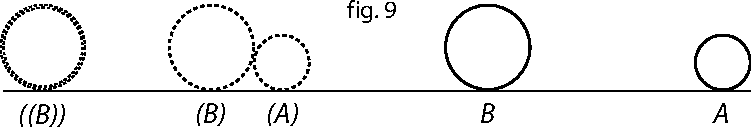
\includegraphics[width=0.72\textwidth]{gesamttex/edit_VIII,3/images/LH_35_09_23_007-008_d.pdf}}%
  \vspace{0.5em}
  \centerline{\lbrack\textit{Fig.~1}\rbrack}\label{LH_35_09_23_008v_Fig.1}%
\newpage
\pstart%
Si%
\edlabel{LH_35_09_23_008v_rcprdpl-1}
nulla alia adessent judicandi
%
\edtext{principia%
\protect\index{Sachverzeichnis}{principium judicandi}
quae excutienda sunt%
\lbrack,\rbrack\
crederem}{%
\lemma{principia}\Bfootnote{%
\textit{(1)}~crederem fore
\textit{(2)}~quae excutienda sunt crederem%
~\textit{L}}}
%
\edtext{%
quietem contingere%
\protect\index{Sachverzeichnis}{quies}
cum ratio reciproca est%
\protect\index{Sachverzeichnis}{ratio reciproca dupla}
%
\edtext{dupla\lbrack:\rbrack\
quoniam enim}{%
\lemma{dupla,}\Bfootnote{%
\textit{(1)}~neque
\textit{(2)}~quoniam enim%
~\textit{L}}}
%
necessario ejus denominator aliquis est numerus
major unitate,
non est cur credatur alius potius quam binarius.%
}{%
\lemma{\textit{Am Rand:}}\Afootnote{%
$ae \, \sqcap \, bi. \;\; \displaystyle\frac{a}{b} \, \sqcap \, \displaystyle\frac{i}{e} \, \sqcap \, \displaystyle\frac{1}{2}$\hspace{5mm} $a\epsilon + by \, \sqcap \,ae+bi\,\sqcap\,4$ \hspace{5mm}$a\epsilon\sqcap 0$%
\textsuperscript{[a]}
et $b\sqcap 2,$ ergo $y\sqcap 2$%
\newline\vspace{-0.5em}%
\newline%
{\footnotesize%
\textsuperscript{[a]}~%
$a\epsilon\sqcap 0$
\textit{(1)}~. Ergo
\textit{(2)}~et%
~\textit{L}\vspace{-3mm}%
% \newline%
}}}
%
Sed hoc argumentum%
\protect\index{Sachverzeichnis}{argumentum}
est praesumtio tantum.%
\protect\index{Sachverzeichnis}{praesumptio generalis}%
%
\edlabel{LH_35_09_23_008v_rcprdpl-2}
Et tunc reperietur
ponendo incurrens quiescere%
\lbrack,\rbrack\
ipsum excipiens%
\protect\index{Sachverzeichnis}{corpus excipiens}
ipsius incurrentis velocitatem%
\protect\index{Sachverzeichnis}{velocitas corporis incurrentis}
assumere,%
\protect\index{Sachverzeichnis}{permutatio velocitatum}
vide%
\protect\index{Sachverzeichnis}{figura}
\edtext{fig.~9.}{%
\lemma{fig.~9}\Cfootnote{%
Das Diagramm \lbrack\textit{Fig.~1}\rbrack\ auf S.~\pageref{LH_35_09_23_008v_Fig.1}.}}
% \pend%
%
%
%\begin{center}     
%\includegraphics[width=0.6\textwidth]{gesamttex/edit_VIII,3/images/lh0370923_008v-d1.pdf}\\
%\rule[0pt]{0mm}{0pt}[\textit{Fig. 1}]
%\end{center}
%
%
% \pstart%
Verum haec praesumtio generalis%
\protect\index{Sachverzeichnis}{praesumptio generalis}
eliditur
per considerationes speciales demonstrativas,%
\protect\index{Sachverzeichnis}{consideratio demonstrativa}
%
\edtext{de
\edtext{quibus
mox.}{%
\lemma{quibus}\Bfootnote{%
\textit{(1)}~post
\textit{(2)}~mox.%
~\textit{L}}}%
}{%
\lemma{de quibus mox}\Cfootnote{%
Gemeint sind wohl die Überlegungen am Anfang der \textit{Scheda IV} (N.~\ref{dcc_04}).%
}}
%
Nunc enim tempus est,
ut in rem omnem accuratius introspiciamus.
\pend%
%
\pstart%
\textls{Si }%
\protect\index{Sachverzeichnis}{corpus minus assequens}%
\protect\index{Sachverzeichnis}{corpus majus}%
\protect\index{Sachverzeichnis}{corpus excipiens}%
\protect\index{Sachverzeichnis}{corpus quiescens}%
\protect\index{Sachverzeichnis}{vis corporis excipientis}%
\protect\index{Sachverzeichnis}{vis corporis incurrentis}%
\protect\index{Sachverzeichnis}{differentia celeritatum}%
\protect\index{Sachverzeichnis}{impulsus}%
\edlabel{LH_35_09_23_008v_sfghj-1}%
%
\edtext{\textls{corpus minus assequatur majus}}{%
\lemma{\textls{corpus}}\Bfootnote{%
\textit{(1)}~\textls{majus assequatur minus}
\textit{(2)}~\textls{minus assequatur majus}%
~\textit{L}}}
%
\textls{necesse est
excipiens ferri primum vi priore,
deinde illa quam accepisset,
si quievisset
et ab incurrente differentia celeritatum fuisset impulsum,
ac denique aliqua alia praeterea.}
Nam si corpus assequatur sibi aequale vel minus,
%
\edtext{ipsi et vim priorem relinquet,%
\protect\index{Sachverzeichnis}{vis relicta}}{%
\lemma{ipsi}\Bfootnote{%
\textit{(1)}~eam vim dabit
\textit{(2)}~et vim priorem relinquet,%
~\textit{L}}}
%
et eam
quam differentia celeritatum%
\protect\index{Sachverzeichnis}{differentia celeritatum}
motum quiescenti dedisset%
\protect\index{Sachverzeichnis}{corpus quiescens}%
\protect\index{Sachverzeichnis}{permutatio velocitatum}
dabit,
et nihil praeterea\lbrack;\rbrack\
nunc vero
quia praeterea
%
\edtext{repellit}{%
\lemma{repellit}\Cfootnote{%
Das Subjekt dieses Prädikats sowie der folgenden \textit{imminuit}, \textit{aufert} und \textit{suscipit} ist nicht mehr der stoßende, sondern der gestoßene Körper.}}
%
incurrens%
\protect\index{Sachverzeichnis}{corpus repulsum}
ideo vim ei superstitem,%
\protect\index{Sachverzeichnis}{vis superstes}
scil. celeritatem utrique communem%
\protect\index{Sachverzeichnis}{celeritas communis}
%
\edtext{qua incurrens%
\protect\index{Sachverzeichnis}{corpus incurrens}
pergere conatur,}{%
\lemma{qua}\Bfootnote{%
\hspace{-0,5mm}incurrens pergere conatur,
\textit{erg.~L}}}
%
imminuit,
quod in prioribus non contigerat,
et eatenus vim aliquam adhuc ei aufert,%
\protect\index{Sachverzeichnis}{vis ablata}
ac proinde
ne ea pereat
in se suscipit.%
\protect\index{Sachverzeichnis}{vis suscepta}
Clarius hoc erit
si inspecta fig.~9%
\protect\index{Sachverzeichnis}{figura}
ponamus \textit{A} et \textit{B} ferri in navi%
\protect\index{Sachverzeichnis}{navis}
mota celeritate \textit{B(A)} vel \textit{B(B)}
et\lbrack,\rbrack\
corpore \textit{B} in navi quiescente%
\protect\index{Sachverzeichnis}{corpus quiescens}%
\lbrack,\rbrack\
in ipsum incurrere \textit{A}
celeritate \textit{AB},
ideo \textit{B} progredietur primum cum navi,%
\protect\index{Sachverzeichnis}{progressus cum navi}
%
\edtext{deinde vi}{%
\lemma{deinde}\Bfootnote{%
\textit{(1)}~celeritate
\textit{(2)}~vi%
~\textit{L}}}
%
velut si quievisset
accepta%
\protect\index{Sachverzeichnis}{vis accepta}
ab \textit{A} celeritate \textit{AB} incurrente%
\protect\index{Sachverzeichnis}{celeritas corporis incurrentis}%
\lbrack;\rbrack\
quia vero
%
\edtext{ipsum \textit{A}}{%
\lemma{ipsum }\Bfootnote{%
\hspace{-0,5mm}\textit{A}
\textit{erg.~L}}}
%
repellit in navi%
\protect\index{Sachverzeichnis}{corpus repulsum in navi}%
\protect\index{Sachverzeichnis}{navis}
%
\edtext{(per priora)}{%
\lemma{(per priora)}\Cfootnote{%
Vgl. N.~\ref{dcc_01}, %??S01\textsubscript{01},
S.~\refpassage{LH_35_09_23_001r_mininmaj-1}{LH_35_09_23_001r_mininmaj-2};
N.~\ref{dcc_02-1}, %??S01\textsubscript{02},
S.~\refpassage{LH_35_09_23_003v_mininmajquies-1}{LH_35_09_23_003v_mininmajquies-2}
}}
%
ac proinde \textit{A} simul ferretur
motibus contrariis,%
\protect\index{Sachverzeichnis}{motus contrarius}
unde vis aliqua destrueretur
in ipso\lbrack,\rbrack\
necesse
%
\edtext{\lbrack erit\rbrack}{%
\lemma{esset}\Bfootnote{%
\textit{L~ändert Hrsg.}}}
%
vim destructam ne%
\protect\index{Sachverzeichnis}{vis destructa}
%
\edtext{pereat,
praeter priores ipsi \textit{B} transferri.%
\protect\index{Sachverzeichnis}{vis translata}%
\edlabel{LH_35_09_23_008v_sfghj-2}}{%
\lemma{pereat,}\Bfootnote{%
\textit{(1)}~communicari
\textit{(2)}~ipsi \textit{B} transferri praeter priores
\textit{(3)}~praeter priores ipsi \textit{B} transferri.%
~\textit{L}}}%
%
\pend%
\count\Bfootins=1200%
\count\Afootins=1200%
\count\Cfootins=1200%
%  \newpage%
%
%
% Ende des Textes auf Blatt 8v
%
%